\section{Results - Scale Testing}
\label{ResultsScaleTesting}
%
The dataset contains several zero-answers, which can happen when subjects doesn't answer on a scale. To exclude some of the zero-points that occured because of a non-answered scale two criterias is stated: 1) If all scale ratings presented on one of the pages are zero, it's probably because subjects skipped a page and 2) If there is a tendency for high ratings on a scale and a zero-answer seems unlikely, it's probably a missing answer.\\

\noindent
The different ratings on the scales in the second test are visualised on \autoref{fig:Boxplot}.
%
\begin{figure}[H]
	\centering
	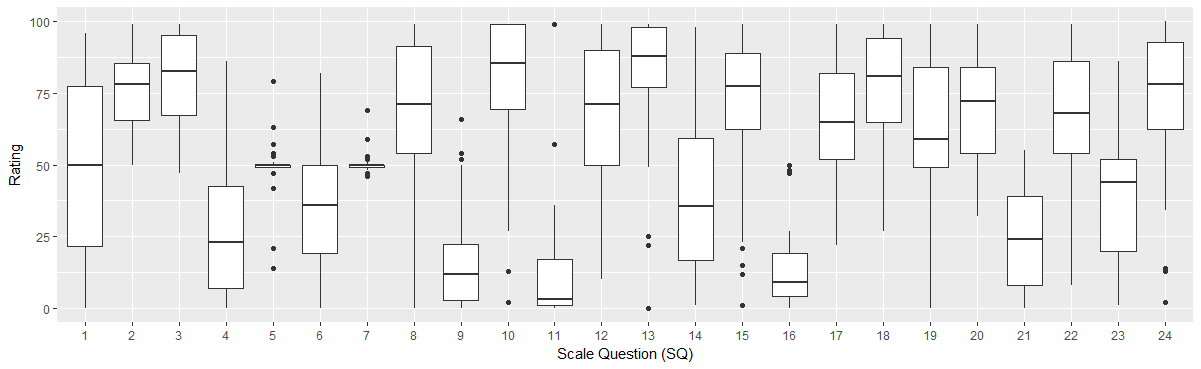
\includegraphics[width = 0.49\textwidth]{Figure/Boksplot24uden0}
	\setlength\abovecaptionskip{-1.2\baselineskip} 
	\caption{Boxplot showing the 24 variables. The boxplot contains a median, the box ranging from 25-75 \% and the whiskers from 0-25 \% and 25-100 \%, respectively.}
	\label{fig:Boxplot}
\end{figure}
\noindent
%
From the boxplots it is seen that the distribution varys. For some SQ, a big part of the scale is used (1, 4, 8, 12, 14, 19), where for xothers a smaller part of the scale is used (2, 3, 5, 7, 9, 11, 13, 16). Furthermore some of the scale ratings looks normal distrubuted (1, 2, 6, 17, 20, 21) and others are skewed (8, 9, 10, 11, 13, 18). In some boxplot data aggregates around midpoints or terminal points (5, 7, 9, 10, 11, 13). SQ5 and SQ7 is centered around the mid point, which can reltate to the label (fine) having to wide a meaning. \\ 

\noindent
When looking at gender differences SQ4 and SQ21 seems to reveal a difference. Women rates SQ4 and SQ21 twice as high as men, which means that they experience the robot's movements more calm but also more intrusive.\\

\noindent
Conducting a PCA on the data results in the screeplot on \autoref{fig:Scree}. It shows that when using 7 dimension only 80 \% of the variance is explained, which is why PCA relating to different groups as the robot's height, distance and direction is conducted. \autoref{fig:biplot} shows the biplot relating to the robot's height. Similar biplots were made for direction and distance.
%
\begin{figure}
	\centering
	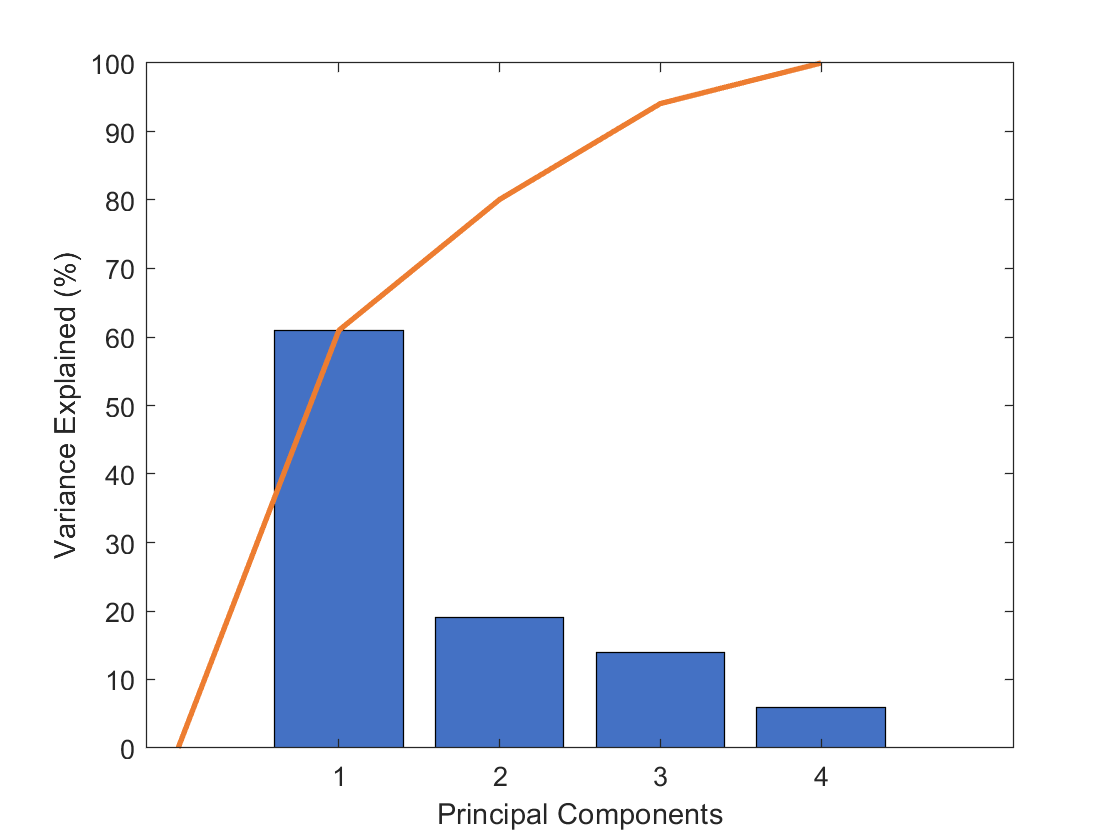
\includegraphics[width = 0.40\textwidth]{Figure/Scree.png}
	\setlength\abovecaptionskip{-1.2\baselineskip} 
	\caption{Scree plot showing the connection between the number of Principal Components and Variance Explained [\%].}
	\label{fig:Scree}
\end{figure}
\noindent
%
\begin{figure}
	\centering
	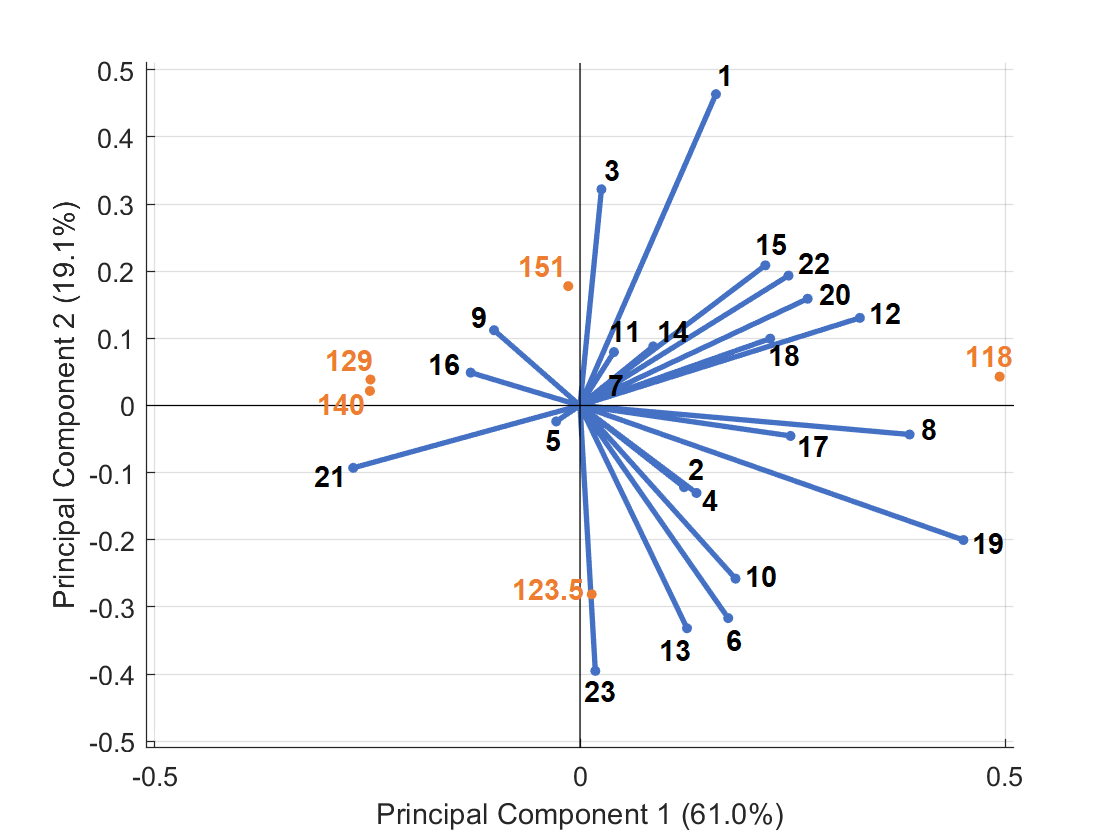
\includegraphics[width = 0.40\textwidth]{Figure/RHeight-Biplot.png}
	\setlength\abovecaptionskip{-1.2\baselineskip} 
	\caption{Biplot showing how the different variables contributes to components and which variables correlates. The black numbers denotes SQ and the red to the different heights in cm.}
	\label{fig:biplot}
\end{figure}
\noindent
%
From \autoref{fig:biplot} it appears that SQ19 contributes the most to PC1 and SQ1 to PC2 relative to the robot's height. Groupings relating to distance shows that SQ1 and partly SQ15 contributes to PC1 and SQ10 contributs to PC2. For direction SQ10 contributes to PC1 and SQ22, and partly SQ1 and SQ20, contributes to PC2. Furthermore 2D and 3D biplots from the different PCAs shows positive and negative correlations between variables/scale questions. These correlations is presented in \autoref{tab:CorrelationsFromPCA}.
%
\begin{table}
	\centering
	\caption{Correlations from PCA}
	\label{tab:CorrelationsFromPCA} 
	\begin{tabular}{ c|c|c }
		\centering
		PCA & Positive correlation & Negative correlation \\ \hline
		\multirow{5}{*}{Height} & SQ8 + SQ17 & SQ2 + SQ9 \\
		& SQ10 + SQ13 & SQ4 + SQ12 \\
		& SQ12 + SQ18 & SQ12 + SQ21 \\
		& SQ14 + SQ15 & SQ16 + SQ19 \\
		&  & SQ18 + SQ21\\ \hline
		\multirow{6}{*}{Distance} & SQ1 + SQ12 & SQ2 + SQ9 \\
		& SQ7 + SQ17 & SQ5 + SQ21 \\
		& SQ8 + SQ21 & SQ10 + SQ13 \\
		& SQ10 + SQ22 & SQ13 + SQ22 \\
		&  & SQ14 + SQ16 \\	
		&  & SQ19 + SQ20 \\ \hline	
		\multirow{5}{*}{Distance} & SQ5 + SQ7 & SQ1 + SQ12 \\
		& SQ8 + SQ10 & SQ6 + SQ23 \\
		& SQ9 + SQ14 & SQ9 + SQ10 \\
		&  & SQ10 + SQ14 \\
		&  & SQ13 + SQ21 
	\end{tabular}        
\end{table}
\noindent
%

To investigate these correlations further ratings from correlating SQ are compared, as seen in \autoref{fig:SQ12+SQ18}. Even though correlations occur when doing PCA on groupings, these comparison doesn't take groupings into consideration. This might be why some correlations isn't found when comparing SQ. From \autoref{fig:SQ12+SQ18} it's seen that the robot is percieved more exciting when subjects like to be served by the robot. Furthermore variables that has a clear correlating from this kind of comparison is shown in \autoref{tab:CorrelationsFromGraphs}.
%
\begin{figure}[H]
	\centering
	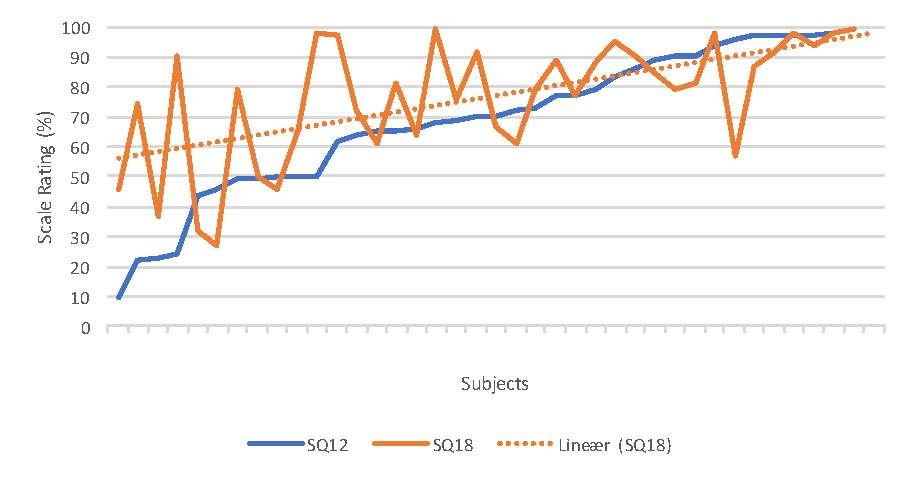
\includegraphics[width = 0.49\textwidth]{Figure/SQ12+SQ18}
	\setlength\abovecaptionskip{-1.2\baselineskip} 
	\caption{Comparison between ratings on SQ12 and SQ18 based on 41 subjects. Two were removed due to incomplete datasets.}
	\label{fig:SQ12+SQ18}
\end{figure}
\noindent
%
\begin{table}
	\centering
	\caption{Correlations from graphs}
	\label{tab:CorrelationsFromGraphs} 
	\begin{tabular}{ c|c }
		\centering
		Positive correlation & Negative correlation \\ \hline
		SQ4 + SQ9 & SQ2 + SQ9 \\ 
		SQ8 + SQ10 & SQ9 + SQ10 \\ 
		SQ8 + SQ17 & SQ12 + SQ21 \\ 
		SQ10 + SQ13 & SQ13 + SQ21 \\ 
		SQ12 + SQ18 & SQ18 + SQ21		
	\end{tabular}        
\end{table}
\noindent
%

In the same manner as comparing SQ with each other the physical parameters can be compared with SQ as well as the demographic parameters. \autoref{fig:HeightSQ6} shows SQ6 compared with the robot's height, which shows that when the robot's height increases the robot is percieved less annoying. Other tendenses seen from theese comparisons is {\color{red} skriv nogle eksempler fra hvordan robotten ellers perciperes med hensyn til demografi.}
%
\begin{figure}[H]
	\centering
	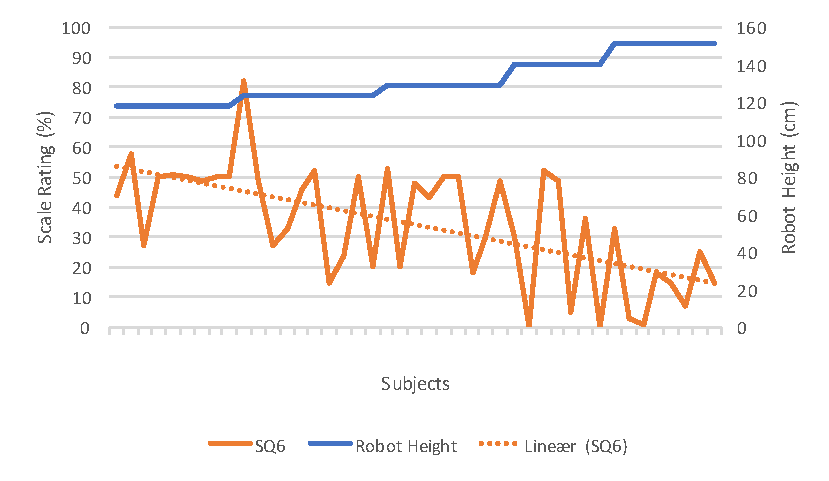
\includegraphics[width = 0.49\textwidth]{Figure/HeightSQ6}
	\setlength\abovecaptionskip{-1.2\baselineskip} 
	\caption{NEW.}
	\label{fig:HeightSQ6}
\end{figure}
\noindent
%